% !Mode:: "TeX:UTF-8" 



\BiSection{2.28}{Figures}

\fancyhead[R]{本题2.28由QC.Z完成}



解:

因为$V_{GS}>V_{TH}$,所以NMOS一定在线性区或饱和区

		\begin{figure}[H] %H为当前位置,!htb为忽略美学标准,htbp为浮动图形
	\begin{minipage}{\linewidth}
		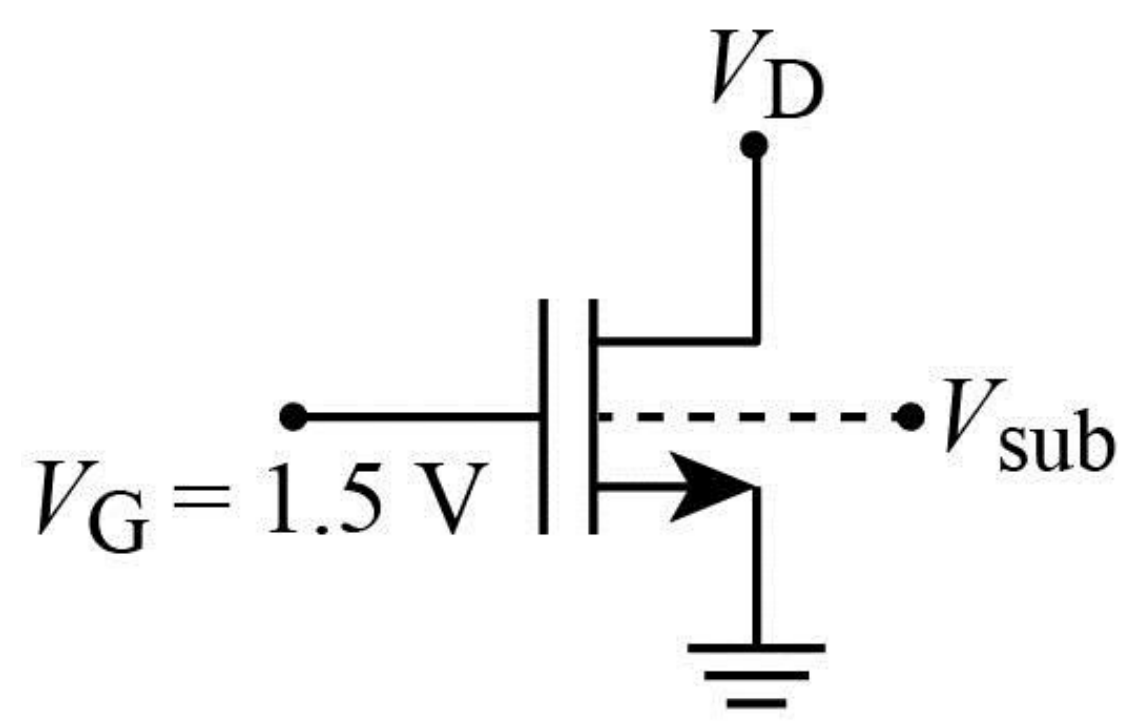
\includegraphics[width=1\linewidth]{2.28-1}
	\end{minipage}
	\caption*{图1} %最终文档中希望显示的图片标题
\end{figure}

对$V_D<0V$:

由图1,如果$V_D<0V$,则源漏交换。当$V_{GS}-V_{TH}>0-V_D$时,NMOS在线性

$V_{TH}=V_{TH0}+\gamma(\sqrt{|2\Phi_F+V_{SB}|}-\sqrt{|2\Phi_F|})$

$|V_{SB}|=|V_S-V_B|$

$V_{TH}=V_{TH0}+\gamma(\sqrt{|2\Phi_F+V_S-V_B|}-\sqrt{|2\Phi_F|})$

$V_{TH}-V_{TH0}=\gamma(\sqrt{|2\Phi_F+V_S-V_B|}-\sqrt{|2\Phi_F|})$

代入$V_S=0$

$V_{TH}-V_{TH0}=\gamma(\sqrt{|2\Phi_F-V_B|}-\sqrt{|2\Phi_F|})$

$\Delta V_{TH}=V_{TH}-V_{TH0}$

$\Delta V_{TH}=\gamma(\sqrt{|2\Phi_F-V_B|}-\sqrt{|2\Phi_F|})$\ding{172}

对$V_{sub}>0V$:

由\ding{172},衬底电压增加导致阈值电压减小,因此漏电流增加
